% !TEX root = diss.tex

\chapter{Do non-redox active metal cations have the potentials to behave as chemo-protective agents? The Effects on Metal Cations on HAT Reaction Barrier Heights}
\label{ch:hat}

\section{Introduction}

Metal cations are ubiquitous in biological systems and play an important role in biological function. As such, there is a great deal of interest in studying metals in biological systems. Proteins in particular are often associated with metals, and in the worldwide Protein Data Bank,\cite{Harding2010, Berman2007} over one-third of crystal structures contain metals. Redox active metals, such as copper and iron, act as co-factors in metalloenzymes for important catalytic processes.\cite{Atkins2010}

Non-redox active metal cations are equally as important in biological function as redox active metals, where they are essential to protein structure and function, along with cellular and neuronal signaling.\cite{Karp1999} Sodium and calcium ions are most abundant extracellurly, while potassium and magnesium are dominant inside of cells. While specific ionic concentrations vary dramatically dependening on physiological conditions, estimates for equilibrium concentrations in both mammalian heart cells\cite{Ingwall2006} and blood plasma\cite{daSilva2001} are listed in~\ref{tab:metalconc}. As sodium and magnesium are most abundant alkali and alkaline earth metals found in biologically relevant systems, they are of prime interest for investigation.

\begin{table}[!htbp]
  \caption{Ionic concentrations inside a mammalian heart cell and in the blood plasma. Concentrations are in units of mM. Values are rounded to one significant figure. Data are from Ref. \protect\citenum{Ingwall2006} and \protect\citenum{daSilva2001}.}
  \label{tab:metalconc}
\begin{tabular}{l c c}
  Ion Conc. & Mammalian Cells & Blood Plasma \\
  \hline
  \ch{Na^+} & 10 & 100--200 \\
  \ch{Mg^{2+}} & 10 & 1 \\
  \ch{K^+} & 100 & 4 \\
  \ch{Ca^{2+}} & 0.1 & 2
\end{tabular}
\end{table}

Extensive crystallographic surveys indicate that metals bind predominantly to oxygen centres in proteins.\cite{Harding1999, Harding2001, Hsin2006} Divalent metals are most often found bound directly to proteins. Calcium binds anywhere from 4 to 6 binding sites in protein crystal structures, while magnesium binds only 1 or 2. Monovalent metals, on the other hand, are often heavily solvated and so they appear in solvent cavities of proteins, although sodium or potassium are sometimes found bound directly to carbonyl or carboxylate oxygen centres.\cite{Harding2010}

A great deal of research has focussed on \ch{Ca^{2+}} in the context of reactive oxygen-centred radical production.\cite{Goerlach2015} Specifically, \ch{Ca^{2+}} ions are important in the mitochondria, where, depending on physiological conditions and concentrations, they can act as inhibitor or promoters of free-radical production in the electron transport chain.\cite{AdamVizi2010} In explanation is that \ch{Ca^{2+}} induce conformational changes of the proteins involved in the electron transport chain which are responsible for radical generation.\cite{Brookes2004} Mitochondrial free-radicals, when present in moderate amounts, can act as cell signalling molecules to activate pro-growth responses.\cite{Sullivan2014} However, ``dysfunctional'' mitochondria can produce excess radicals leading to oxidative damage which has been linked to degenerative diseases.

Given the significant importance alkali and alkaline earth metals play in biological systems, their impact on protein oxidation must be considered. However, until recently, kinetic studies of protein oxidation have not investigated the mechanistic role of non-redox active metals. In a series of three papers,\cite{Salamone2013a, Salamone2015metals, Salamone2016} Bietti and colleagues have shown that alkali and alkaline earth metals have an inhibitory effect on HAT reactions involving oxygen radicals and organic substrates. The experimental results of these papers are summarized in~\ref{tab:hat-metals}. All results are from time-resolved LFP in nitrogen or argon-saturated acetonitrile (MeCN) at 298 K, as was previously described in section~\ref{sec:hat-methods}. Experiments also demonstrate that metal cations increase the rate of $\beta$-scission decay of \cumo,

\begin{table}
  \caption{Table summary of experimental data - Needs completion}
  \label{tab:hat-metals}
  \begin{tabular}{l l c c}
    Substrate & Conditions & $k_H$ & $k_H$(MeCN)/$k_H$(M$^{n+}$) \\
    \hline
    1,4-cyclohexadiene &  & 6.7\E{7} & \\
    (CHD)  & \ch{LiClO4} 1.0 M & 7.5\E{7} & 0.89 \\
     & \ch{Mg(ClO4)2} 1.0 M & 7.0\E{7} & 0.96 \\
    tetrahydrofuran &  & 5.7\E{6} & \\
    (THF) & \ch{LiClO4} 1.0 M & 2.9\E{6} & 1.7 \\
     & \ch{LiOTf} 1.0 M & 2.8\E{6} & 2.0 \\
     & \ch{Mg(ClO4)2} 1.0 M & 1.8\E{6} & 3.2 \\
    triethylamine &  & 2.0\E{8} & \\
    (TEA) & \ch{LiClO4} 1.0 M & 9.4\E{7} & 2.1 \\
     & \ch{Mg(ClO4)2} 0.005 M & $<$1\E{6} & $>$200 \\
    1,2,2,6,6-pentamethylpiperidine &  & 1.7\E{8} & \\
    (PMP) & \ch{LiClO4} 1.0 M & 9.0\E{7} & 1.9 \\
     & \ch{Mg(ClO4)2} 0.005 M & $<$1\E{6} & $>$170 \\
    $N,N$-dimethylformamide & & 1.2\E{6} & \\
    (DMF) & \ch{LiClO4} 0.5 M & $k_{H1}$ = 8.9\E{5} & 1.3 \\
      & & $k_{H2}$ = 1.5\E{6} & 0.80 \\
      & \ch{NaClO4} 0.2 M & $k_{H1}$ = 9.6\E{5} & 1.3 \\
      & & $k_{H2}$ = 1.4\E{6} & 0.86 \\
      & \ch{Mg(ClO4)2} 0.2 M & $k_{H1}$ =
    $N,N$-dimethylacetamide & &
  \end{tabular}
\end{table}

Firstly, rate constants for

\section{Computational methods and details}

All quantum mechanical calculations were performed using the Gaussian 09 software package,\cite{Frisch2009} or the TURBOMOLE software package.\cite{turbomle} Calculations for the benchmark quality data to test metal binding to substrates were first optimized at the LC-$\omega$PBE-D3(BJ)/6-31+G(2d,2p) level of theory, and later re-optimized with larger 6-311+G(3df,3pd) basis sets. Single-point energy calculations were then carried out using the CCSD(T) methodology and various basis sets, as described in Section~\ref{sec:benchmark}. Final benchmark quality binding energies have been calculated using the F12$^*$ explicitly correlated method with Def2-QZVPPD primary basis sets and Def2-QZVPP auxiliary basis sets required for the resolution-of-the-identity approximation as implemented in TURBOMOLE, which is used to reduce the computational cost associated with calculating MO integrals.\cite{note-book} DFT-based methods were tested both by single-point energy calculations on the benchmark structures, and by geometry optimization starting from the benchmark structures.

To test the effects of metal cations on HAT barrier heights, calculations were first performed the reactions not involving metal cations. Geometry optimizations were performed at the M05-2X/6-31+G$^{**}$ level of theory. Transition state (TS) structure optimization was performed by first freezing the acceptor-hydrogen-donor bond lengths with multiple initial orientations. The frozen bonds were then relaxed to give the final TS structure, which was then used to identify the pre- and post-reaction complexes associated with tat TS structure. All structures were verified minima (or saddle-points with a single imaginary frequency connecting reactants to products for TS structures) by harmonic frequency calculation. Single-point energy calculations were performed at the M05-2X/6-311+G(2d,2p) level of theory. The effects of MeCN solvent were estimated by inclusion of the SMD continuum solvent model in single-point energy calculations. Geometry optimizations were also performed for all reactions, however many calculations failed to converge.

The inclusion of metal cations proved to be technically very challenging. 



\section{Benchmarking Density Functional Theory Based Methods for the Binding of Alkali and Alkaline Earth Metals to Organic Substrates and Oxygen Centred Radicals}

\subsection{Background}

In order to study the central hypothesis proposed in this work, we must carefully select a computational method. In particular, we wish to use density-functional theory (DFT), which is known to be prone to various problems such as self-interaction error \cite{Dutoi2006}, delocalization error,\cite{OterodelaRoza2014} and the inability to treat non-covalent interactions.\cite{Johnson2009,DiLabio2016} The latter of these can be corrected by the selection of a method capable correcting the non-covalent corrections such as a pair-wise dispersion model \jnote{\textbackslash-cite{D3}}, or atom centered potentials developed by our group \jnote{\textbackslash-cite{DCPS}}. Other errors can be ignored through the careful selection of a DFT method.

We are interested in selecting a method which can accuratetly treat the interactions between alkali and alkaline earth metal cations, and organic substrates and radicals. To this end, there exists little literature, with one notable paper\cite{Suarez2011} which examines the binding of calcium cations to organic substrates. In this paper, \citet{Suarez2011} provide accurate energetic, electronic, and structural results for the binding of calcium to organic neutral and charged species, as well as assess the performance of four different DFT methods. They also analyze the nature of ligand-metal bonding interactions using a symmetry-adapted perturbation theory approach (SAPT) \jnote{EXPAND ON THIS}

Due to our interest in alkali and alkaline earth metal cations in FHT, we determined it necessary to prepare benchmark quality data for binding to organic substrates and radicals.

\jnote{Calcium prefers to bind to O, with binding to S or N is
  rare\cite{Harding1999}} In N,N-dimethylacetamide for example, calcium
  binds preferentially to the lone pairs of the carbonyl oxygen over
  the nitrogen lone pair. This is shown in \ref{fig:DMA-Ca}.

  \begin{scheme}[hbt]
    \centering
    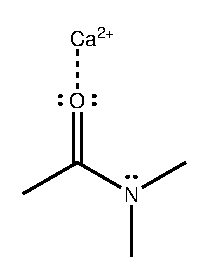
\includegraphics{figures/DMA-Ca.eps}
    \caption{Binding of the calcium cation (\ch{Ca^{2+}}) to the
      oxygen lone pairs of N,N-dimethylacetamide.}
    \label{fig:DMA-Ca}
  \end{scheme}



\subsection{Methods}

Conformers were generated using Hyperchem with the AM1 semi-empirical molecular orbital (MO) method \jnote{\textbackslash-cite{hyperchem}} followed by optimization calulations of 5-10 lowest energy structures using at the \jnote{(currently unpublished)} BLYP-D3/pc1 level of theory, including our own groups basis set incomplete potential (BSIPs).\jnote{(CITATIONS)}

On the basis of the work by \citet{OterodelaRoza2014}, which showed that in systems which are halogen bonded, erroneous charge transfer can be significant, and given the charge on the metal cations, the LC-$\omega$PBE density functional with D3 dispersion correction and moderate 6-31+G(2d,2p) \jnote{(CITATIONS for DFT and D3)} basis sets were applied to determine the most strongly bound complexes of substrates and metal cations. Global minima monomers and complexes were optimized with the LC-$\omega$PBE-D3 method near the basis set limit (6-311+G(3df,3pd).  Highly correlated wavefunction results were obtained at the CCSD(T) level of theory with extrapolation to the complete basis set limit.\jnote{CITATION} Calculations were performed using the Gaussian 09 package\cite{Frisch2009}, and wavefunction calculations were performed using the TURBOMOLE\cite{turbomole} package.


\subsection{Benchmark systems}

The purpose of this work is to provide high-level binding energies for organic substrates which are of interest directly for this project, but also which may be useful for future work. The substrates proposed were to be relevant to simple biological models such as dipeptide like molecules and the hydroxyl and hydroperoxyl radical. We also wanted to incorporate substrates with are important to the physical organic experiments that are performed to probe these systems, thus solvents such as acetonitrile and dimethyl sulfoxide and the benzyloxyl and cumyloxyl radicals were also included. This set is shown in \ref{fig:set1}\jnote{FIND CDX}.

\begin{scheme}[hbt]
  \centering
    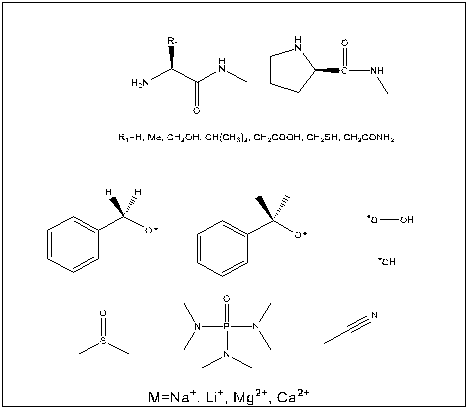
\includegraphics{figures/set1}
    \caption{Initial proposed benchmark set of molecules and cations. Note this set consistes of all combinations of substrates and metal cation, thus there are 60 complexes in the set.}
  \label{fig:set1}
\end{scheme}

Benchmark quality binding energies are generally calculated using the ``gold standard'' approach, CCSD(T)/CBS, where correlation consistent basis sets\jnote{(CITATION)} (cc-pV\emph{X}Z, \emph{X}=T,Q,5) developed by Dunning and co-workers are used for complete basis set extrapolation. These basis sets have limited availability for the metals of interest. Specifically, basis sets for K are note available, and only non-augmented basis sets for Li, Na, Mg, and Ca. It is necessary to include core correlation of the n-1 shell in alkali and alkaline earth metals, thus it is advantageous to use core valence basis sets such as cc-pCV\emph{X}Z. These basis sets are even more limitted, thus we opted for the augmented version of the polarization consistent basis sets of Jensen and co-workers (aug-pc-\emph{N}, \emph{N}=2,3,4). \jnote{CITATIONS FOR GOLD STANDARD AND BASIS SETS, NEED THEORY SECTION ON DIFFERENT BASIS SETS}

While performing CCSD(T)/CBS calculations, we notices that the metal cations (and neutral metal atoms), did not converge smoothly to the complete basis set limit. Given this, and the limitted computational resources, we decided to re-evaluate the size scope of the benchmark set being used. In order to facilitate future DFT work and probe the issue of basis set convergence of alkali and alkaline earth metals, a benchmark set of small substrates was proposed. This new set is shown in \ref{fig:set2}. The new, small benchmark set was selected to include important functional groups and radicals for biological systems and the most common solvent used in physical organic experiments, acetonitrile.

\begin{scheme}[hbt]
  \centering
    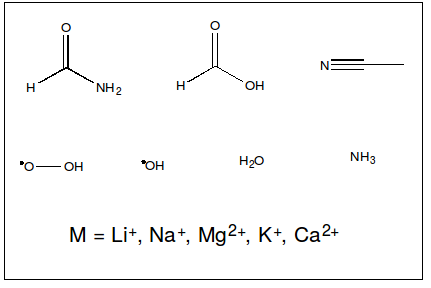
\includegraphics{figures/set2}
    \caption{Revised benchmark set of small substrates and cations. Note this set consistes of all combinations of substrates and metal cation, thus there are 35 complexes in the set.}
  \label{fig:set2}
\end{scheme}

\subsection{Metal cation basis set convergence}

\subsection{High level results and evaluation of various density-functional theory methods}
